\documentclass[a4paper,10pt]{scrartcl}
\usepackage[utf8]{inputenc}
\usepackage{amsmath}
\usepackage{algorithm}
\usepackage{algpseudocode}
\usepackage{tikz}
%opening
\title{CSC418 Assignment 1}
\author{Philip Lee - 9999074932}
\setlength{\parindent}{0cm}
\begin{document}

\maketitle


\section{Parametric Equations}
$x(t) = 4\cos{2\pi t} + 1/16 * \cos{32\pi t} \\ y(t) = 2\sin{2\pi t} + 1/16 * \sin{32\pi t}$

\subsection{Tangent Vector}

The tangent vector is given by $p(t) = <\frac{dx}{dt}, \frac{dy}{dt}>$\\
$ p(t) = <-8\pi\sin{2\pi t} - 2\pi\sin{32\pi t}$ , $ 4\pi\cos{2\pi t} + 2\pi\cos{32\pi t}>$

\subsection{Normal Vector}

The normal vector $n(t)$ will satisfy $p(t) \cdot n(t) = 0$ so therefore $n(t) = <- \frac{dy}{dt}, \frac{dx}{dt}>$
$ n(t) =  < - 4\pi\cos{2\pi t} - 2\pi\cos{32\pi t}$, $-8\pi\sin{2\pi t} - 2\pi\sin{32\pi t}>$

\subsection{Symmetry}

{\bfseries The curve is not symmetric about the y axis.}\\

{\bfseries Counter Example:}\\

If we evaluate at $t = 1/8$,  $<x(1/8), y(1/8)> = <4/\sqrt{2} + 1/16, 2/\sqrt{2}>$\\
For the curve to be symmetric about the y axis and by the definition of symmetry,
there must exist a value of $t_o$ such that
\[<x(t_o), y(t_o)> = <-(4/\sqrt{2} + 1/16), 2/\sqrt{2}>\]

It turns out that $y(t_o) = 2/\sqrt{2}$ only for $t_o = 1/8, 3/8$ \\\\
The presence of only two solutions for $t_o$ can be justified by inspecting
the plots of $f(t) = 2/\sqrt{2} - 1/16\sin{32\pi t}$ and $g(t) = 2\sin{2\pi t}$

Evaluating $x$ at $t_o$ gives $x(3/8) = -4\sqrt{2} + 1/16$ \\

Since $x(3/8) \neq -x(1/8)$ and $y(3/8) = y(1/8)$ the curve is not symmetric about the y axis because. There is a point on the curve that
cannot be reflected about the y-axis.\\\\


{\bfseries The curve is symmetric about the x axis.}\\

{\bfseries Proof:}\\

For every value of $t_o$, there must exist a value $t_1$ such that  
\[ <x(t_o), y(t_o)> = <x(t_1), -y(t_1)>\]

To demonstrate this, let us consider the parametric function on the interval of \\$-1/2 < t < 1/2$\\

Recall that an odd function has the property that $f(t) = -f(-t)$ and that an even
function has the property $f(t) = f(-t)$. Also, the sum of two even functions is even, and the sum of
two odd functions is also odd.\\

Since $x(t)$ is the sum of two cosines which are even functions, $x(t)$ is even about $t = 0$.
Since $y(t)$ is the sum of two sines which are odd functions, $y(t)$ is odd about $t = 0$.\\

Consider an arbitrary $t_o$ in the range $0 < t_o < 0.5$. Since $x(t)$ is an even function, $x(t_o) = x(-t_o)$.
Since $y(t)$ is an odd function, $y(t_o) = -y(-t_o)$. \\

Thus for any given $t_o, 0 < t_o < 0.5$, choosing $t_1 = -t_o$ satisfies the condition for symmetry about the y axis.

\[ <x(t_o), y(t_o)> = <x(t_1), y(t_1)>\]\\
\[ = <x(-t_o), y(-t_o)>\]\\
Which by the even and odd properties of the functions $x(t), y(t)$ \\ 
\[ = <x(t_o), -y(t_o)>\]\\

Since the range of $t$ covers the entire curve, this implies that the curve is symmetric about the x-axis.
\subsection{Curve's Perimeter}

The formula to compute the curve's perimeter is given by

\[ L = \int_{a}^{b} \sqrt{\left( \frac{dx}{dt}\right)^2 + \left( \frac{dy}{dt}\right)^2}dt\]

The limits must be over one complete period. Since $x(t)$ has period $1$ and $y(t)$ has period $1$ the limits of the integral can be $a=0$ and $b=1$

Taking the derivatives from $p(t)$, we get

\[ L = \int_{0}^{1} \sqrt{\left( -8\pi\sin{2\pi t} - 2\pi\sin{32\pi t} \right)^2 + \left( 4\pi\cos{2\pi t} + 2\pi\cos{32\pi t}\right)^2}dt\]

This integral is pretty tedious to solve analytically.

\subsection{Curve's Perimeter Approximation}

The perimeter can be piecewise approximated by dividing the curve into even segments,
and finding the sum of the lengths of each segment which is a straight line. The smaller the segments,
the more accurate the approximation will be.\\

For example, we know that the curve exists for the interval $0 < t < 1$. Divide the curve into $k$ segments where $k$ is an integer greater than 0.
Then evaluate $p(t)$ at $t = nT$, where $n = 0,1,2 \ldots k-1$ and $T = 1/k$. Then find the cartesian distance between
$p(nT)$ and $p((n+1)T)$ for all $n$ and take the sum. Thus the final formula becomes:\\
\[
\sum_{n=0}^{k-1}
  ||\,p(nT) - p((n+1)T)||,\,\] where $k$ is the number of piecewise segments and $T = 1/k$

\section{Intersections of a 2D Line And Circle}

\subsection{Area of Grey Region}

The area of the grey region is given by \[ A = \pi(r_2-r_1)^2\]

\subsection{Number of Intersections}

There can be :

\begin{itemize}
 \item $0$ Intersections
 \item $1$ Intersection if the line is tangent to the larger circle
 \item $2$ Intersections if the line passes through the larger circle but does not intersect with the inner circle
 \item $3$ Intersections if the line passes through the larger circle and is tangent to the inner circle
 \item $4$ Intersections if the line passes through both circles and is not tangent to the inner circle
\end{itemize}

\subsection{Determine Number of Intersections}

The number of locations can be computed analytically as follows:

Consider the number of times the line intersects with a circle $r$.\\

We are given that $\bar p(\lambda) = \bar p_o + \lambda\bar d$ and the equation of the circle is given by \\$||\bar q - \bar p_1 ||^2 = r^2$\\

An intersection with the circle means that there is some value of $\lambda$ for $\bar p(\lambda)$ that satisfies the equation of the circle. Thus we can substitute $\bar p(\lambda)$.\\

\[||\bar q - \bar p(\lambda)||^2 = r^2\]\\

Expanding and simplifying the equation and finding the magnitude of the vectors:

\[||\bar q - (\bar p_o + \lambda\bar d) || ^2 = r^2\]
\[\sqrt{ (q_x - p_{ox} - \lambda\bar d_x)^2 +  (q_y - p_{oy} - \lambda\bar d_y)^2}^2  = r^2\]\\

Since $q_x, q_y, p_{ox}, p_{oy}$ are given (center of circle and one point on the line), let $\Delta_x = q_x - p_{ox}$ and $\Delta_y = q_y - p_{oy}$

\[(\Delta_x - \lambda\bar d_x)^2 +  (\Delta_y - \lambda\bar d_y)^2  = r^2\]\\

Expanding and grouping terms:
\begin{equation}
 \lambda^2(d_x^2 + d_y^2) + 2\lambda(\Delta_xd_x + \Delta_yd_y) + ((\Delta_x^2 + \Delta_y^2) - r^2) = 0
\end{equation}
The number of solutions can be determined by looking at the discriminant. If the discriminant is negative, there are no intersections between the line and this circle.
If the discriminant is positive, there are two intersections between the line and this circle. If the discrimant is zero, there is one intersection.\\

The discriminant is given by: 

\[ b^2-4ac = (\Delta_xd_x + \Delta_yd_y)^2 - 4(d_x^2 + d_y^2) ((\Delta_x^2 + \Delta_y^2) - r^2) \]

{\bfseries Thus, the number of intersections between the line and the donut can be achieved by evaluating the discriminant for circles $r = r_1$ and $r = r_2$ and summing the result.}

\subsection{Location of Intersections}

The location of the intersections can be determined by determining the roots of equation $(1)$ for the circles with $r = r_1$ and $r = r_2$. The location can be solved by
using the quadratic formula which gives a value for $\lambda_o$.

\[ \lambda_o = \frac{-(\Delta_xd_x + \Delta_yd_y) \pm \sqrt{(\Delta_xd_x + \Delta_yd_y)^2 - 4(d_x^2 + d_y^2) ((\Delta_x^2 + \Delta_y^2) - r^2)}}{2(d_x^2 + d_y^2)}\]

with $\Delta_x = q_x - p_{ox}$ and $\Delta_y = q_y - p_{oy}$\\

This $\lambda_o$ can then be substituted into $p(\lambda)$ to determine the intersections.


\subsection{Intersections After Non-Uniform Scaling Line and Circle}

If both the line and circle are scaled non-uniformly by the same transformation, then the number of intersections remains the same. \\

Consider a circle and line that intersects at a point $\bar p_o$. Thus $p_o$ must lie on the circle. When the circle is scaled with reference to the origin, that point on the circle will become\\

\[\bar p_1 = \begin{bmatrix}
    s_x       & 0 & 0 \\
    0       & s_y & 0 \\
    0       & 0 & 1     
 \end{bmatrix} \bar p_o\]
 
 The point $p_o$ must also lie on the line. When the line is scaled, the point on the line will map to
 
 \[\bar p_2 = \begin{bmatrix}
    s_x       & 0 & 0 \\
    0       & s_y & 0 \\
    0       & 0 & 1     
 \end{bmatrix} \bar p_o\]
 
 
Since $\bar p_o = \bar p_1$, the intersection will still exist after the transformation. A similar argument can be made for points that do not intersect will not intersect after the transformation. Thus
the number of intersections before and after will remain the same.\\

However, the locations of the intersections will change according to the scaling values about the origin. As demonstrated above, the new intersection location will be given by $p_1$\\

\subsection{Intersections After Non-Uniform Scaling Circle Only}

If the circle is scaled non-uniformly, then the number of intersections will change completely along with the locations of the intersection. A new implicit equation for the circle would have to be chosen
and locations solved similar to how equation (1) was derived.\\

To demonstrate why the number of intersections and locations will change unpredictably, consider the following example.\\

Imagine a circle centered at $(0,5)$ with a radius $r = 1$ and a line with equation $y = 3$. The point $(0, 4)$ lies on the circle. There are no intersections between between the line and circle.\\

If the circle is scaled by a factor of $s_x = 1, s_y = 5$, then the point $(0,4)$ will map to $(0, 20)$. There are still no intersections between the line and circle.\\

If the circle is scaled by a factor of $s_x = 1, s_y = 0.75$, then the point $(0,4)$ will map to $(0, 3)$. There is one intersections between the line and circle.\\

If the circle is scaled by a factor of $s_x = 1, s_y = 0.25$, then the point $(0,4)$ will map to $(0, 1)$. There will be two intersections between the line and circle that now have an $x$ value not one.\\

Though this was shown for only one circle, it applies also for the two circles that form the donut with $r = r1$ and $r = r2$



\section{Do Transforms Commute?}

\subsection{Translation and Uniform Scaling}

The translation and uniform scaling transforms do not commute in general.

Consider the transformation matrix \\

$T = 
\begin{bmatrix}
    1       & 0 & t_x \\
    0       & 1 & t_y \\
    0       & 0 & 1 
\end{bmatrix}
$, where $t_x $ and $t_y$ are the translations in the $x$ and $y$ direction. \\

and the uniform scaling matrix \\

$S_{Uniform} = \begin{bmatrix}
    s       & 0 & 0 \\
    0       & s & 0 \\
    0       & 0 & 1     
 \end{bmatrix}
$, where $s$ is the scaling factor. \\

Scaling first then translating. Multiplying the two matrices $T$ and $S$ gives: \\

$T \bullet S_{Uniform} = \begin{bmatrix}
		  s & 0 & t_x \\
		  0 & s & t_y \\
		  0 & 0 & 1
               \end{bmatrix}
$ \\

Translating first then scaling gives: \\

$S_{Uniform} \bullet T = \begin{bmatrix}
		  s & 0 & st_x \\
		  0 & s & st_y \\
		  0 & 0 & 1
               \end{bmatrix}
$ \\ 

These transformations matrices are not the same for $s \neq 1$ and thus the transforms do not commute. \\ 

{\bfseries{Example:}}

Consider the point $P_o = \begin{bmatrix} 1 \\ 1 \end{bmatrix}$, a transformation of $t_x = -1$ and $t_y = -1$ and a scaling $s = 2$\\
Applying the translation first gives $P_{1a} = \begin{bmatrix} 0 \\ 0 \end{bmatrix}$ \\ 
Appling scaling second gives $P_{1b} = \begin{bmatrix} 0 \\ 0 \end{bmatrix}$

Reversing the order of the transforms:

Applying scaling first gives $P_{2a} = \begin{bmatrix} 2 \\ 2 \end{bmatrix}$ \\
Applying translation second gives  $P_{2b} = \begin{bmatrix} 1 \\ 1 \end{bmatrix}$ \\

$P_{2b} \neq P_{2a}$

\subsection{Translation and Non-Uniform Scaling}


{\bfseries The translation and non-uniform scaling transforms do not commute in general.}

Consider the transformation matrix \\

$T = 
\begin{bmatrix}
    1       & 0 & t_x \\
    0       & 1 & t_y \\
    0       & 0 & 1 
\end{bmatrix}
$, where $t_x $ and $t_y$ are the translations in the $x$ and $y$ direction. \\

and the non-uniform scaling matrix \\

$S_{Non\_Uniform} = \begin{bmatrix}
    s_x       & 0 & 0 \\
    0       & s_y & 0 \\
    0       & 0 & 1     
 \end{bmatrix}
$, where $s_x$ and $s_y$ are the scaling factors. \\

Scaling first then translating. Multiplying the two matrices $T$ and $S_{Non\_Uniform}$ gives: \\

$T \bullet S_{Non\_Uniform} = \begin{bmatrix}
		  s_x & 0 & t_x \\
		  0 & s_y & t_y \\
		  0 & 0 & 1
               \end{bmatrix}
$ \\

Reversing the order of the transformation gives: \\

$S_{Non\_Uniform} \bullet T = \begin{bmatrix}
		  s_x & 0 & s_xt_x \\
		  0 & s_y & s_yt_y \\
		  0 & 0 & 1
               \end{bmatrix}
$ \\ 

These transformations matrices are not the same for $s_x \neq 1$ and $s_y \neq 1$ and thus the transforms do not commute.

\subsection{Rotation and Scaling}

Consider a rotation and scaling about the same fixed point about the origin. {\bfseries This transformation commutes for uniform scaling where $s_x = s_y$. Otherwise the transformation does not commute.}\\

{\bfseries Proof:}

The scaling matrix is given by \\

$S_{Non\_Uniform} = \begin{bmatrix}
    s_x       & 0 & 0 \\
    0       & s_y & 0 \\
    0       & 0 & 1     
 \end{bmatrix}
$, where $s_x$ and $s_y$ are the scaling factors. \\

The rotation matrix is given by \\

$R = \begin{bmatrix}
      \cos{\theta}       & -\sin{\theta} & 0 \\
      \sin{\theta}       & \cos{\theta} & 0 \\
      0       & 0 & 1             
     \end{bmatrix}
$   , where $\theta$ is the rotation

Doing a scale followed by a rotation gives: \\

$R \bullet S_{Non\_Uniform} = \begin{bmatrix}
		  s_x\cos{\theta} & -s_y\sin{\theta} & 0 \\
		  s_x\sin{\theta} & s_y\cos{\theta} & 0 \\
		  0 & 0 & 1
               \end{bmatrix}
$ \\


Doing a rotation followed by a scale gives: \\

$S_{Non\_Uniform} \bullet R = \begin{bmatrix}
		  s_x\cos{\theta} & -s_x\sin{\theta} & 0 \\
		  s_y\sin{\theta} & s_y\cos{\theta} & 0 \\
		  0 & 0 & 1
               \end{bmatrix}
$ \\

These transformation matrices are equivalent only if $s_x = s_y$. Thus this transform does not commute in general.

\subsection{Scaling About Different Fixed Points}

{\bfseries The transformations of scaling about different fixed points do not commute.} As a counter example, consider 
the point $P_o = \begin{bmatrix} 1 \\ 1 \end{bmatrix}$, a scaling $S_1$ of $s_x = 1$ and $s_y = 2$ about the origin
$\begin{bmatrix} 0 \\ 0\end{bmatrix}$, and a scaling $S_2$ of $a_x = 3$ and $a_y = 3$ about $P_r = \begin{bmatrix} 0 \\ 1\end{bmatrix}$\\\\


{\bfseries Case 1}: $S_1$ followed by $S_2$.\\
If we first apply $S_1$ with respect to origin, we get $P_{1a} = \begin{bmatrix} 1 \\ 2 \end{bmatrix}$\\
If we then apply $S_2$ with respect to $P_r$, we get $P_{1b} = \begin{bmatrix} 3 \\ 4\end{bmatrix}$\\

{\bfseries Case 2:} $S_2$ followed by $S_1$.\\
If we first apply $S_2$ with respect to $P_r$, we get $P_{2a} = \begin{bmatrix} 3 \\ 1\end{bmatrix}$\\
If we then apply $S_1$ with respect to origin, we get $P_{2b} = \begin{bmatrix} 3 \\ 2\end{bmatrix}$\\

Since $P_{2b} \neq P_{1b}$ the two transforms do not commute.

\subsection{Translate and Shear}

{\bfseries The transformations of translating and shear do not commute.}

Consider the transformation matrix \\

$T = 
\begin{bmatrix}
    1       & 0 & t_x \\
    0       & 1 & t_y \\
    0       & 0 & 1 
\end{bmatrix}
$, where $t_x $ and $t_y$ are the translations in the $x$ and $y$ direction. \\

and the shear matrix \\

$S_{Shear} = \begin{bmatrix}
    1       & s_y & 0 \\
    s_x       & 1 & 0 \\
    0       & 0 & 1     
 \end{bmatrix}
$, where $s_x, s_y$ is the shear factor. \\

Shearing first then translating. Multiplying the two matrices $T$ and $S$ gives: \\

$T \bullet S_{Shear} = \begin{bmatrix}
		  1 & s_y & t_x \\
		  s_x & 1 & t_y \\
		  0 & 0 & 1
               \end{bmatrix}
$ \\

If however, we apply the translation matrix first followed by the shear matrix gives:

$S_{Shear} \bullet T = \begin{bmatrix}
		  1 & s_y & s_xt_x \\
		  s_x & 1 & s_yt_y \\
		  0 & 0 & 1
               \end{bmatrix}
$ \\

These transformations matrices are not the same for $s_x, s_y \neq 1$ and thus the transforms do not commute. \\ 


{\bfseries{Example:}}

Consider the point $P_o = \begin{bmatrix} 1 \\ 1 \end{bmatrix}$, a transformation of $t_x = -1$ and $t_y = -1$ and a shear of $s_x = 2, s_y = 3$\\
Applying the translation first gives $P_{1a} = \begin{bmatrix} 0 \\ 0 \end{bmatrix}$ \\ 
Appling shear second gives $P_{1b} = \begin{bmatrix} 0 \\ 0 \end{bmatrix}$

Reversing the order of the transforms:

Applying shear first gives $P_{2a} = \begin{bmatrix} 4 \\ 3 \end{bmatrix}$ \\
Applying translation second gives  $P_{2b} = \begin{bmatrix} 3 \\ 2 \end{bmatrix}$ \\

$P_{2b} \neq P_{1b}$ so the transforms do not commute.

\section{Triangles}

\subsection{Is point q inside or outside triangle}

Recall that in Bresenham's line algorithm, a point can be determined to be above or below a parametrized straight line.

\begin{algorithm}[h!]
  \caption{Is Point Above or Below Line}\label{}
  
  \begin{algorithmic}
    \Function{F}{Point $p$, Parametrized Line}
    \State{$x \gets p_x, y \gets p_y$}
    \State{$f(x,y) = (xdy - ydx) \gets $ Parametrized Line}\\
    \If{$f(x,y) < 0$}
    \State Point above line
    \ElsIf{$f(x,y) > 0$}
    \State   Point below line
    \Else 
    \State Point on line
    \EndIf\\
    \EndFunction
    
  \end{algorithmic}
\end{algorithm}

   
\begin{algorithm}[h!]
  \caption{Point Inside or Outside Triangle}\label{}
  \begin{algorithmic}
    \State Given vertices of triangle $\bar v_1, \bar v_2, \bar v_3$
    \State Given point $\bar q$
    \State Parametrize the lines between $\bar v_1, \bar v_2$ and $\bar v_1, \bar v_3$ and $\bar v_2, \bar v_3$
    \State Count $\gets 0$
    \For{Each parametrized line $l$}
      \State Check if point $\bar q$ lies above or below $l$ using Algorithm 1
      \State To determine if that point lies on the 'inside' of the triangle, check that the result
      for point $\bar q$ matches the result for the point not used to parametrize the line 
      \State Example: If $\bar v_1$ and $\bar v_2$ were used to parametrize the line, check whether $\bar v_3$ lies above or below $l$ and compare
      that to the result of $\bar q$
      \If{Result of $\bar q$ matches result of third point}
	\State Count$++$
      \EndIf
    \EndFor
    
    \If{Count $== 3$}
      \State Point lies in triangle.
    \Else
      \State Point lies outside triangle.
    \EndIf  
  \end{algorithmic}
\end{algorithm}

\newpage

\subsection{Is point q on edge of triangle}

To determine if a point is on the edge of a triangle, perform a check similar to the previous part, but use
the fact that if Algorithm 1 evaluates to $0$, the point is on the line. See Algorithm 3.


\begin{algorithm}[h]
  \caption{Point Inside or Edge of Triangle}\label{}
  \begin{algorithmic}
    \State Given vertices of triangle $\bar v_1, \bar v_2, \bar v_3$
    \State Given point $\bar q$
    \State Parametrize the lines between $\bar v_1, \bar v_2$ and $\bar v_1, \bar v_3$ and $\bar v_2, \bar v_3$
    \State Count $\gets 0$
    \State PointOnLine $\gets False$
    \For{Each parametrized line $l$}
      \State Check if point $\bar q$ lies above or below $l$ using Algorithm 1
      \State To determine if that point lies on the 'inside' of the triangle, check that the result
      for point $\bar q$ matches the result for the point not used to parametrize the line i.e. if
      $\bar v_1$ and $\bar v_2$ were used to parametrize the line, check whether $\bar v_3$ lies above or below
      \\
      {\bfseries
      \State If Algorithm 1 returns a 0, that does not necessarily mean that $\bar q$ lies on the edge. It simply means
      that $\bar q$ lies on the parametrized line. For the line to be on the edge of the triangle,
      $\bar q$ must lie on the 'correct' side of the triangle, by checking if the signs match in the same manner
      as Algorithm 2}
      \Comment{Modifaction from prior part}
      \\
      \If{Signs match}
	\State Count$++$
      \EndIf
      
      \If{\Call{F}{$\bar q$, $l$} ==  Point On Line}
	\State PointOnLine $\gets True$
      \EndIf
    \EndFor
    
    \
    \If{Count $== 2 $ \&\& PointOnLine $==$ True}
      \State Point lies on edge of triangle.
    \Else
      \State Point lies inside or outside triangle.
    \EndIf  
  \end{algorithmic}
\end{algorithm}

\newpage


\subsection{Triangulate Quadrilateral}

A quadrilateral has four vertices, $A, B, C, D$. To triangle the quadrilateral as two triangles, simply create
a triangle from $ABC$, and a second triangle from $BCD$

\subsection{Triangulate N-Sided Convex Polygon}

A convex polygon means that no angle in the polygon is greater than $180 ^o$. A property of a convex polygon is that
a straight line can be drawn from one vertex to every vertex in the polygon.

If the vertices of the polygon are given by $V_1, V_2, \dots, V_n$ and are in counter clockwise order
,then the shape can be triangulated by connecting $(V_1, V_2, V_3)$ then $(V_1, V_3, V_4) \dots (V_1, V_{n-1}, V_{n})$

\subsection{Triangulate Concave Polygon}

Consider the following shape. There is no single vertex where a line can be drawn to every other vertex.
Thus the above triangulation procedure will not work. Examples are drawn in dashed red and cyan lines.

\begin{figure}[!h]
 \centering
 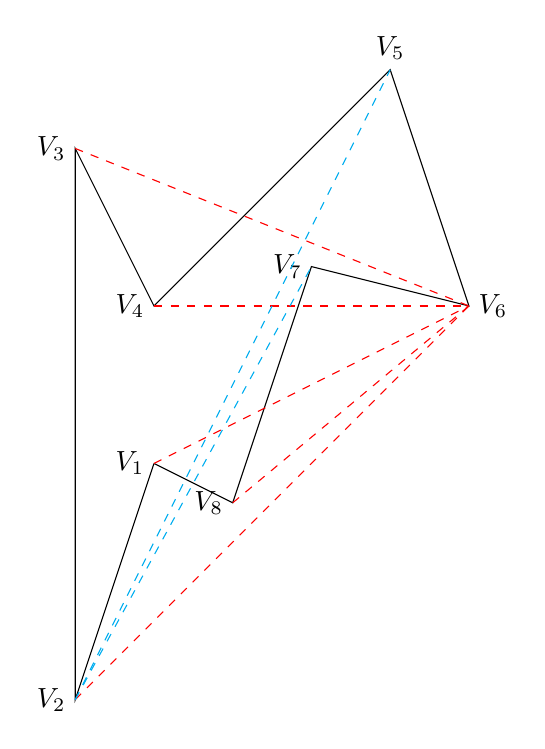
\begin{tikzpicture}
  
    \draw (0,0) -- (-1,-3) -- (-1, 4) -- (0, 2) -- (3, 5) -- (4, 2) -- (2, 2.5) -- (1, -0.5) -- (0,0);
    \node [left] at (0,0){$V_1$};
    \node [left] at (-1,-3){$V_2$};
    \node [left] at (-1,4){$V_3$};
    \node [left] at (0,2){$V_4$};
    \node [above] at (3,5){$V_5$};
    \node [right] at (4,2){$V_6$};    
    \node [left] at (2,2.5){$V_7$};        
    \node [left] at (1,-0.5){$V_8$};        
    
    %V6
    \draw[dashed, red] (-1, -3) -- (4,2);
    \draw[dashed, red] (0, 0) -- (4,2);    
    \draw[dashed, red] (1, -0.5) -- (4,2);        
    \draw[dashed, red] (0, 2) -- (4,2);            
    \draw[dashed, red] (-1, 4) -- (4,2);                
    
    %V2
    \draw[dashed, cyan] (-1, -3) -- (3,5);            
    \draw[dashed, cyan] (-1, -3) -- (2,2.5);                    
 \end{tikzpicture}

 \caption{Concave polygon that does not work with the above triangulation procedure.}
 
\end{figure}

\newpage
\subsection{Determine if Point In/Out of Convex Polygon}


\begin{algorithm}[!h]
  \caption{Point Inside or Outside or On Convex Polygon}\label{}
  \begin{algorithmic}
    \State Triangulate the polygon
    \State NumOutside $\gets 0$, NumInside $\gets 0$, NumEdge $\gets 0$
    \For{Each triangle $t$}
      \State Check if point is inside, outside, or on triangle
      
      \If{Inside}
	\State NumInside$++$
      \ElsIf{Outside}
	\State NumOutside$++$
      \Else
	\State NumEdge$++$
      \EndIf
    \EndFor
    
    \If{NumEdge $== 1$}
      \State Point is on edge 
      \Comment Note that the point could be inside the polygon but still on the triangles edge. If this is the case,
      then the the number of times the point was on the edge will be greater than 1, since the triangles on the interior of
      the polygon share an edge with another triangle
    \ElsIf{NumInside $> 1$ $||$ NumEdge $ > 1$}
      \State Point is on inside
      \Comment If the point was inside a single triangle, then it must lie inside the polygon. This also
      covers the case where the point was on the edge of a triangle but inside the polygon in which case NumEdge$ = 2  $
    \Else
      \State Point is on outside
    \EndIf
  \end{algorithmic}
\end{algorithm}

\end{document}
